
\section*{一、实验目的与原理}


\subsection*{1. 实验目的}

测量电流计内阻，利用分流、分压电阻将其改装成单量程 5 mA 电流表和 5 V 电压表，并用标准表校验示值、评定等级；组装欧姆表，观察电流与待测电阻的关系，理解欧姆刻度的非均匀性。

\subsection*{2. 电流计内阻与电流表改装}

电流计满偏电流为 $I_g=1\,\mathrm{mA}$，内阻为 $R_g$。替代法保持电源及其他电阻不变，用电阻箱替换电流计，调至回路电流恢复原值，电阻箱读数即为表头内阻。中值法在电流计两端并联电阻，并保持总电流不变，调至电流计半偏，此时并联电阻等于表头内阻。

\begin{figure}[H]\centering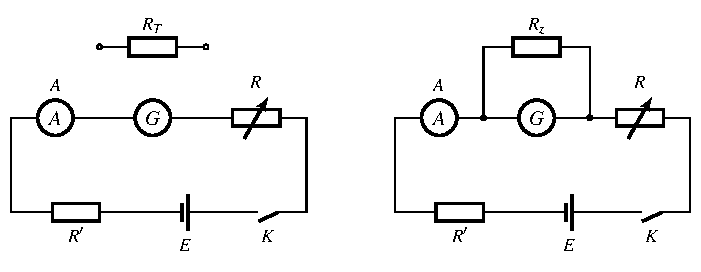
\includegraphics[width=.96\linewidth,height=3.5cm,keepaspectratio]{circuits/preliminary.pdf}\caption{电流计内阻测量：替代法与中值法}\end{figure}

本次课堂采用单量程电路，只需在表头两端并联一个分流电阻 $R_1$。由两支路电压相等，

\[
I_gR_g=(I_m-I_g)R_1,\qquad R_1=\frac{I_gR_g}{I_m-I_g}=\frac{R_g}{4},\quad I_m=5\,\mathrm{mA}.
\]

改装表示值 $I_G$ 为原电流计示值的五倍。校验时改装表与标准安培表串联，比较同一回路电流下的两表示值。

\begin{figure}[H]\centering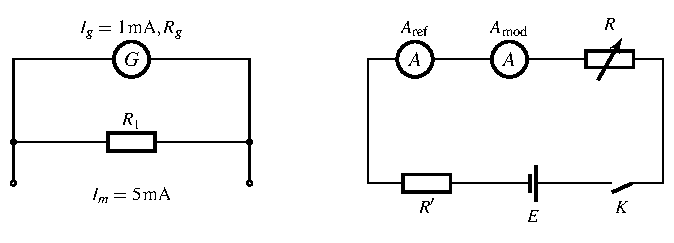
\includegraphics[width=.96\linewidth,height=3.5cm,keepaspectratio]{circuits/single-ammeter.pdf}\caption{单量程电流表设计与校验电路}\end{figure}

\newpage
\subsection*{3. 电压表改装}

保留改装电流表的分流支路，将其作为等效表头。其满偏电流 $I'_g=5\,\mathrm{mA}$，等效内阻为

\[
R'_g=\frac{R_gR_1}{R_g+R_1}.
\]

串联分压电阻 $R_3$ 后，满偏电压满足

\[
(R_3+R'_g)I'_g=5\,\mathrm V,\qquad R_3=1000\,\Omega-R'_g.
\]

校验时将改装表与标准伏特表并联，比较同一电压下的两表示值。

\begin{figure}[H]\centering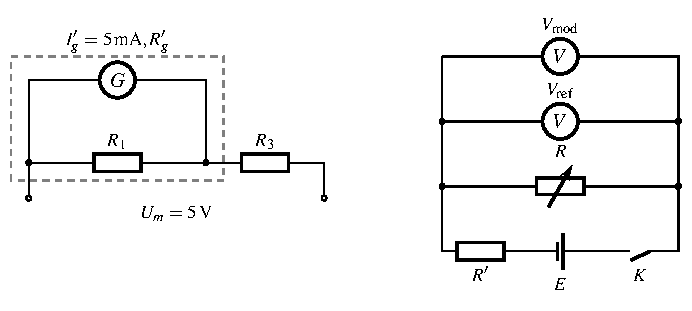
\includegraphics[width=.96\linewidth,height=3.5cm,keepaspectratio]{circuits/single-voltmeter.pdf}\caption{单量程电压表设计与校验电路}\end{figure}

\subsection*{4. 欧姆表原理}

本次欧姆表保留电流表的并联分流支路，使用一节 1.5 V 电池和 220 Ω 保护电阻。短接调零时，原电流计指针满偏为 1.00 mA，改装电流表的满偏总电流为 5 mA。欧姆表利用内置电源使电流通过待测电阻。短接表笔调零后，记表头满偏示值为 $I_0$、从测量端口看入的等效内阻为 $R_0$，在电源和接线保持不变时有

\[
\frac{I_x}{I_0}=\frac{R_0}{R_0+R_x},\qquad R_x=R_0\left(\frac{I_0}{I_x}-1\right).
\]

短接时 $R_x=0$，指针满偏；开路时 $R_x\to\infty$，电流趋于零；半偏时 $R_x=R_0$。电阻与电流不是线性关系，电阻刻度从大到小的方向与电流刻度相反，高阻端密、低阻端疏。

\begin{figure}[H]\centering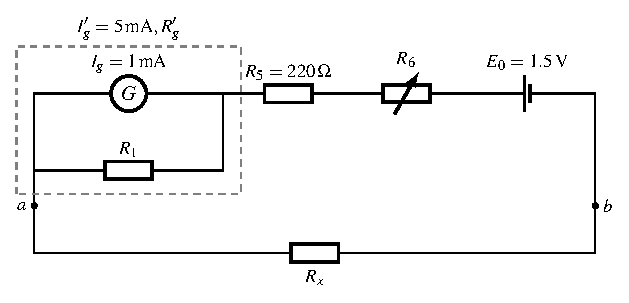
\includegraphics[width=.96\linewidth,height=3.5cm,keepaspectratio]{circuits/actual-ohmmeter.pdf}\caption{实际欧姆表电路：保留并联分流支路}\end{figure}
